\chapter{Implementation Plan} 
% Main chapter title

\label{Chapter5} 
%Call reference to this chapter use \ref{ChapterX}

\lhead{Chapter 5. \emph{Implementation Plan}} 
% Change X to a consecutive number; this is for the header on each page - perhaps a shortened title

\doublespacing
% LINE FORMATTING

%\clearpage
%\pagebreak

\section{Project Task Identification}

\subsection{Identification of Critical Success Factors}

Critical success factors are a key requirement which is necessary and essential to be identified to achieve the project objectives in this project. The requirement for our design objectives are listed below: 


\begin{enumerate}
\item \textbf{Determine a suitable operating system.} The operating system should be reliable, secure and appropriate for data processing, concurrent and distributed computing activities. If the selected operating system does not meet requirements, a new operating system has to be considered.

\item \textbf{Acquire free public data set for big data processing.} Large data set is required for data processing with concurrent and distributed computing to make use of concurrent programming language’s package and architecture. If the data set obtains not clean and useful, data cleansing and data deduplication have to be conducted.

\item \textbf{Selection of database management system (DBMS). } The database-management system for this project should support for operating system, concurrent programming language and project activities. If the selected DBMS does not compatible and suitable, a new DBMS capability has to be considered. 

\item \textbf{Installation and setup DBMS for big data handling.} The selected database-management system should be installed and running on the operating system for data storing and data handling. The database system allows developer to conduct development activities for manage concurrency control for update and retrieval in this project.

\item \textbf{Selection of Go and RUST concurrent programming language for comparison. } There are many types of concurrent programming language for system development. The selected language for this project is RUST and Go. This programming language architecture, packages and capabilities should be considered to conduct performance comparison.

\item \textbf{Coding of “Import CSV into database” with Go program.} The program is required to write with Go language to read CSV and upload into PostgreSQL database. This task is conduct for data definition and data preparation before data processing is performed. 

\item \textbf{Coding of “Import CSV into database” with RUST program. } The program is required to write with Go language in order to read CSV and upload into PostgreSQL database. This task is conduct for data definition and data preparation before data processing is performed. 

\item \textbf{Conduct minor comparison on sequential and concurrent programming with Go and RUST language on PostgreSQL database transaction.} The sequential and concurrent program is required to write with Go and RUST language in order to conduct a comparison of execution time for database retrieval on PostgreSQL.

\item \textbf{Conduct minor comparison on sequential and concurrent programming with Go and RUST language on reading CSV files. } The sequential and concurrent program is required to write with Go and RUST language to conduct a comparison of execution time on reading CSV files.


\end{enumerate}

\pagebreak

\subsection{Project Tasks for FYP Phase 1}

\begin{enumerate}[topsep=0pt,itemsep=-1ex,partopsep=1ex,parsep=1.5ex]
	
\item Installation of Ubuntu 16.04 LTS 64-bit operating system.
\item Acquire free public data set for big data processing.
\item Installation of  Eclipse Parallel Application IDE Parallel Oxygen version. 
\item Selection of Go and RUST concurrent programming language for comparison.
\item Installation of Go language compiler and Goclipse plugin for Eclipse IDE.
\item Installation of RUST language compiler and RustDT plugin for Eclipse IDE.
\item Selection of PostgreSQL object-oriented relational database management system (OORDBMS).
\item Installation and setup PostgreSQL database system intro PC for data handling.
\item Golang programming for import CSV files into PostgreSQL database.
\item Sequential and concurrent programming with Golang on PostgreSQL database retrieval.
\item Sequential and concurrent programming with Golang on reading CSV files.
\item Big data checking, cleaning and preparation with Data Validation. 

\end{enumerate}

\begin{landscape}
	\subsection{Gantt Chart for Phase 1}
	\begin{figure}[H]
		\centering
		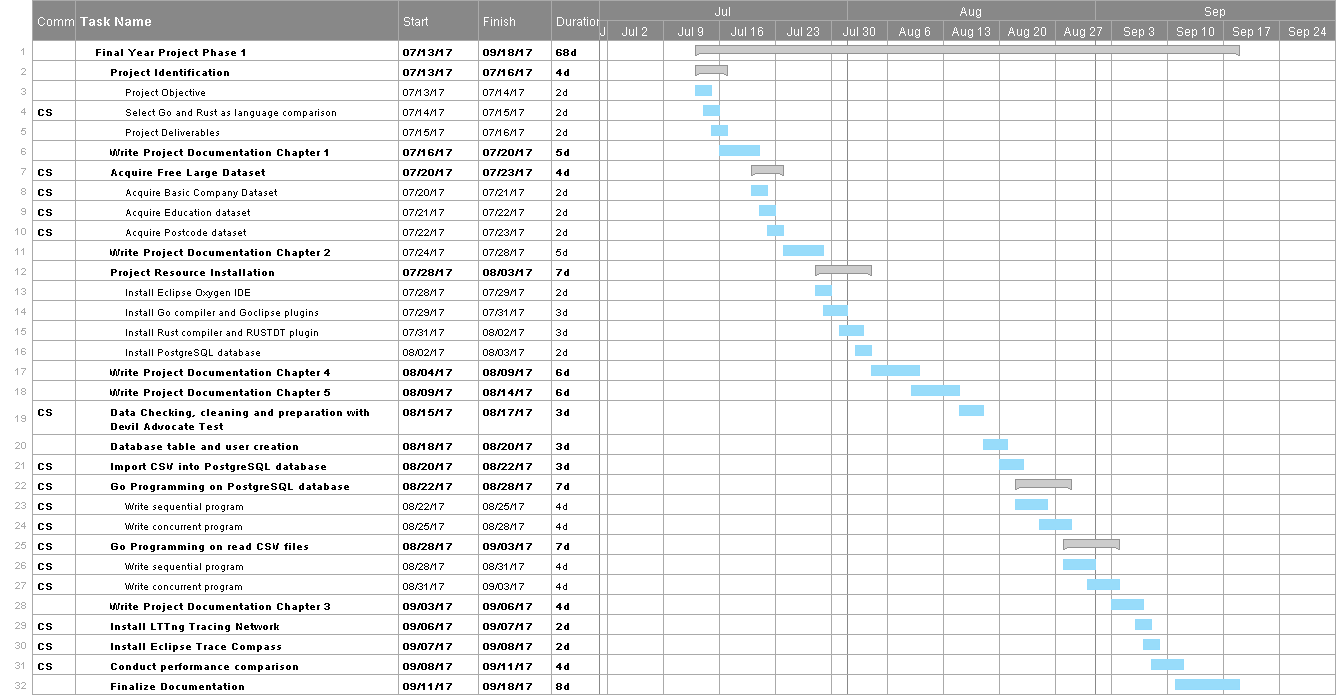
\includegraphics[width=1.5\textwidth]{Figure/Gantt1.png}
		\rule{35em}{0.5pt}
		\caption[Gantt Chart for Phase 1]{Gantt Chart for Phase 1}
	\end{figure}
\end{landscape}

\subsection{Project Tasks for FYP Phase 2}

\begin{enumerate}[topsep=0pt,itemsep=-1ex,partopsep=1ex,parsep=1.5ex]
	\item Data encoding.
	\item Data transformation. 
	\item Data parsing. 
	\item Data cleansing. 
	\item Data normalization.
	\item Database tuning. 
	\item Query tuning. 
	\item Data migration.
	\item Sequential and concurrent programming with Go and RUST on PostgreSQL database retrieval.
	\item Sequential and concurrent programming with Go and RUST on reading CSV files.
	
\end{enumerate}

\begin{landscape}
	\subsection{Gantt Chart for Phase 2}
	\begin{figure}[H]
		\centering
		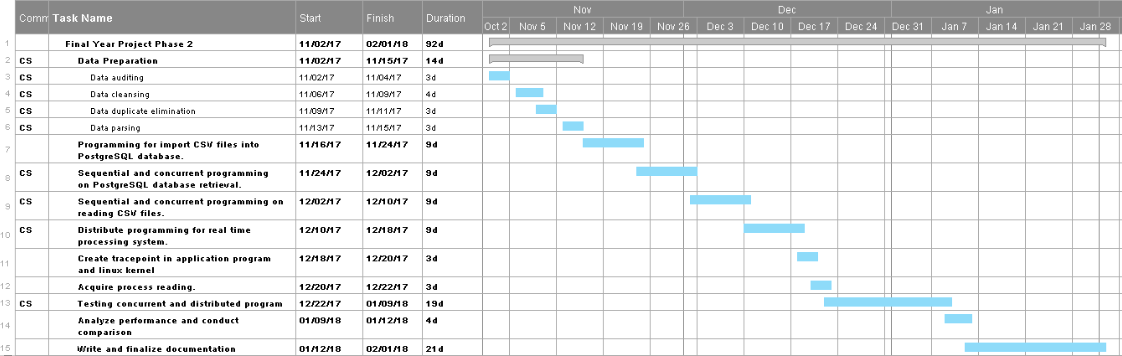
\includegraphics[width=1.5\textwidth]{Figure/Gantt2.png}
		\rule{35em}{0.5pt}
		\caption[Gantt Chart for Phase 2]{Gantt Chart for Phase 2}
	\end{figure}
\end{landscape}


\subsection{Milestone Deliverables}
The milestone deliverables are:

\begin{enumerate}[topsep=0pt,itemsep=-1ex,partopsep=1ex,parsep=1ex]
\item Go program for data parsing, object relational mapping and data migration. 
\item RUST program for data parsing and object relational mapping.
\item PL/pgSQL's DDL and DML scripts for database creation, manipulation and migration control.
\item A report based of this project. 
\end{enumerate}

%MAIN SECTION ================================
\section{Planned Execution Activities}

\subsection{Phase 1}

\begin{enumerate}[topsep=0pt,itemsep=-1ex,partopsep=1ex,parsep=1.5ex]
	
	\item \textbf{Data Validation.}
	 The Data Validation is conducted to ensure obtained raw CSV data set is clean and useful. The expected result of this test is the number of commas in the record should not exceed the number of columns in a database. In addition, the data content itself should be unique and suitable for storing in the database. More information is provided in Appendix B.1.
		
	\item \textbf{Golang programming for import CSV files into PostgreSQL database.}
	The Golang programming for import CSV raw data into PostgreSQL is to ensure Go language is capable of processing raw CSV data and PostgreSQL database. The expected result for this program should read 100 rows of data from raw CSV file and insert into PostgreSQL database. More information is provided in Appendix C.
	
	\item \textbf{Sequential and concurrent programming with Golang on PostgreSQL database retrieval.}
    The Go program should retrieve 300 rows of data from three tables (each table 100 rows) in PostgreSQL database sequentially and concurrently. The expected result for this program is concurrent processing should have better performance than sequential. More information is provided in Appendix D.	
	
	\item \textbf{Sequential and concurrent programming with Golang on reading CSV files.}
	The Go program should retrieve 100 rows of data from raw CSV file sequentially and concurrently. The expected result for this program is concurrent processing should have better performance than sequential. More information is provided in Appendix E.
	 
\end{enumerate}

\subsection{Phase 2}

\begin{enumerate}[topsep=0pt,itemsep=-1ex,partopsep=1ex,parsep=1.5ex]
	
	\item \textbf{Data encoding.}
	This activity is a deliverable of Phase 2 in this project. It is conducted to ensure that the dirty and corrupted datasets are converted into consistent format so that it will be safe to used for Object Relational Mapping, Data Transformation and Data Parsing. More information is provided in Appendix J.1 to J.2. 
	
	\item \textbf{Development of PL/pgSQL scripts for data transformation.} 
	This activity is a deliverable of Phase 2 in this project. It is conducted to extract data in CSV format from raw datasets and import into PostgreSQL database. More information is provided in Appendix K.1 to K.2.
	
	\item \textbf{Development of Go and Rust Object Relational Mapping (ORM) program for data retrieval.}
	This activity is a deliverable of Phase 2 in this project. The data from CSV file and PostgreSQL database are retrieved and map into object model. Go and Rust program should retrieve 4 millions row of data from raw CSV file and PostgreSQL database in sequential and concurrent manner. The execution duration of each program are tabulated and recorded for comparison purposes. 
	More information is provided in Appendix L.1 to L.4.
	
	\item \textbf{Development of PL/pgSQL DDL scripts for normalized entity creation.}
	This activity is a deliverable of Phase 2 in this project. It can eliminate redundancy and data anomalies to improve data integrity. Database design is performed to define table and establish relationship between entity to create a relational database schema. Moreover, normalized table will be created correctly with PL/pgSQL's DDL scripts based on the Entity Relationship Diagram shown in Section 3. More information is provided in Appendix M.
	
	\item \textbf{Development of Go data parser program.}
	This activity is a deliverable of Phase 2 in this project. The missing fields will be eliminated and data standardization is conducted to promote conformity and usability of data. More information is provided in Appendix N.1.
	
	\item \textbf{Database tuning.}
	This activity is a deliverable of Phase 2 in this project. It is performed to configure PostgreSQL's database environment and setting to increase performance on data processing. More information is provided in Appendix O.
	
	\item \textbf{Development of PL/pgSQL's DML scripts and Go concurrent program for database migration.}
	This activity is a deliverable of Phase 2 in this project. The data that are transformed and cleaned will be import into normalized table. These data are migrated from legacy storage into new storage within PostgreSQL database. More information is provided in Appendix P.1.
	
\end{enumerate}

